\documentclass[11pt]{article}
\usepackage[utf8]{inputenc}
\usepackage{graphicx}
\usepackage{a4wide}
\usepackage[square, numbers]{natbib}
\usepackage{algpseudocode}
\usepackage{boxedminipage}
\usepackage{amsthm}
\usepackage{amsmath}
\usepackage{amsfonts}
\usepackage{amssymb}
\usepackage{tikz}
\usepackage{multirow}

\usepackage[
bookmarks=true,
colorlinks=true,
breaklinks=true,
urlcolor=red,
citecolor=blue,
linkcolor=blue,
unicode=true,
]
{hyperref}

%\renewcommand*\rmdefault{iwona}

\paperwidth=210 true mm
\paperheight=297 true mm
\pdfpagewidth=210 true mm
\pdfpageheight=297 true mm

\author{Daniel Meister and Ji\v{r}i Bittner}
\title{Time-Varying Appearance}

\begin{document}

\begin{center}
\textsc{\LARGE Time-Varying Appearance}\\[0.4cm]
\textsc{\Large Technical Report - February 2018}\\[0.4cm]
\textsc{\large Toyota Research Lab}\\[0.4cm]
\textsc{\normalsize Daniel Meister and Ji\v{r}i Bittner}\\[0.5cm]
\end{center}

\section{Introduction}

\section{Related Work}

\paragraph{Weathering:} Traditionally, various phenomena have been studied individually weathering effects and proposed models based on physically inspired simulations: metallic patinas \cite{Dorsey1996a}, flow of water \cite{Dorsey1996b}, stone weathering \cite{Dorsey1999,Xue2011}, lichen growth \cite{Desbenoit2004}, peeling and cracking \cite{Paquette2002}, dust accumulation \cite{Hsu1995}, scratches \cite{Bosch2004}, stains \cite{Bosch2011}, and wet surfaces \cite{Nakamae1990,Jensen1999}. Chen et al.~\cite{Chen2005} proposed a general simulation based on tracing weathering particles similar to photon mapping. In last decade, data-driven models became popular. Lu et al.~\cite{Lu2006} proposed a data-driven parametric model of drying effect. Gu et. al~\cite{Gu2006} proposed a general non-linear factorization of spatial and temporal components of the phenomena modeling various phenomena. Similarly, Sun et al.~\cite{Sun2007} studied more complex time-varying phenomena such as drying of paints and dust accumulation; however, this approach is not spatial varying. Wang et al~\cite{Wang2006}, Xue et al.~\cite{Xue2008}, Bandeira and Walter~\cite{Bandeira2009}, and Bellini et al.~\cite{Bellini2016} proposed methods based on capturing data at a single time instant from which extract the effect using non-linear dimensionality reduction tools.

% \cite{Wong1997}, \cite{Georghiades2005}, \cite{Lu2007}

\paragraph{Texture Synthesis:} Efros et al.~\cite{Efros2001} proposed texture synthesis based on region growing when a synthesized texture is assembled from small \emph{quilts}. Kwatra et al.~\cite{Kwatra2005} formulated texture synthesis problem as a minimization of energy function iteratively improving the synthesized texture in global manner. Fi\v{s}er et al.\cite{Fiser2016} proposed to use texture synthesis to stylize 3D rendering using additional channels to guide the synthesis based-on global illumination. Barnes et al.~\cite{Barnes2009} proposed an efficient randomized algorithm for searching nearest neighbors between patches which is a common problem in texture synthesis. Texture synthesis algorithms were traditionally designed to use only static RGB channels. Tong et al.~\cite{Tong2002} extended texture synthesis for BTF. Enrique et al.~\cite{Enrique2005} suggested how to measure distance between time-varying parameters.

\section{Space-Time Varying Factorization (STAF)}
We will recall the STAF model proposed by Gu et al.~\cite{Gu2006}. The measured data are fit into the combination of Lambertian and simplified Torance-Sparrow model:
\begin{equation}
\rho(x,y,\vec{\omega}_i, \vec{\omega}_o, t) = K_d(x,y,t) + \frac{K_s(x,y,t)}{4(\vec{\omega}_i \cdot \vec{n})(\vec{\omega}_o \cdot \vec{n})}\exp\left[-\left(\frac{\vec{\omega}_h \cdot \vec{n}}{\sigma(x,y,t)}\right)^2\right],
\end{equation}
where $\vec{\omega}_i$ and $\vec{\omega}_o$ are incoming and outgoing direction, $\vec{n}$ is the surface normal, and $\vec{\omega}_h$ is the half-angle vector. The BRDF parameters are the diffuse intensity $K_d$ (RGB color), the specular intensity $K_s$, and the surface roughness $\sigma$. Each parameter is dependent on spatial location $(x,y)$ and time $t$. Each of the BRDF parameters $p$ is factorized into 5 factors:
\begin{equation}
p(x,y,t) = A(x,y)\phi(t')+B(x,y),
\end{equation}
\begin{equation}
t'=R(x,y)t-O(x,y),
\end{equation}
where $\phi(t')$ is the \emph{temporal characteristic curve}, the \emph{rate} $R(x,y)$ and the \emph{offset} $O(x,y)$, and the time invariant $A(x,y)$ and $B(x,y)$. Intuitively, the temporal characteristic curve is common for all pixels corresponding to the particular  phenomenon (e.g. drying) assuming that the parameters of all pixels are similar in some sense. However, different pixels differs in both time and spatial domains. The factors $R$ and $O$ describe how pixels evolve in different locations in time. The factors $A$ and $B$ describe time invariant features of the material. For example, we can change the underlying texture by modifying the $A$ and $B$. The authors provided the publicly available database containing 20 samples of various phenomena - burning, drying, decay, and corrosion (see Figure~\ref{Fig:Database}). 

\begin{figure}[htb] 
\begin{center}
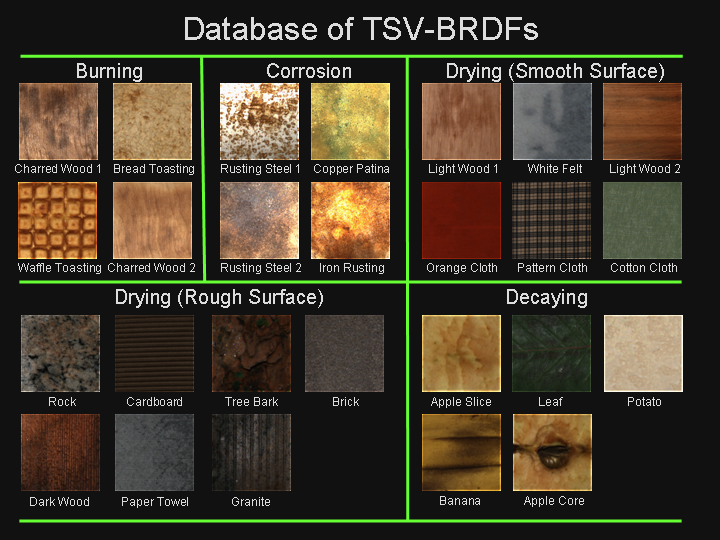
\includegraphics[width=0.75\textwidth]{figures/database}
\end{center}
\caption{The STAF database contains various phenomena \cite{Gu2006}.}
\label{Fig:Database}
\end{figure}

\section{TSV-BRDF Synthesis}
The goal of the example-based texture is an enlargement of the texture, i.e. synthesize larger texture from small example However, it is not obvious how to extend texture synthesis not only for TSV-BRDF but also for SV-BRDF since we work with functions instead of constant values for each pixel. Simple solution is to use the texture synthesis algorithm with channels corresponding to 20 STAF factors, i.e. four factors for each BRDF parameter. The problem is that the BRDF parameters have different scales and different. Generally, surface roughness $\sigma$ is by two orders of magnitude larger than diffuse or specular intensities. This issue might be solved by normalization of parameters; however, the parameters have also different influence on the reconstructed BRDF model. Similarly, the STAF factors have difference scales and different influence on a reconstructed BRDF parameter. The temporal characteristic curve $\phi$ is polynomial different for each BRDF parameter. For example, rate $R$ and offset $O$ have different influence on the reconstructed parameter. To measure distance correctly, we must measure directly between BRDF of RGB channels similarly to traditional texture synthesis. We can measure distance between BRDF using $L_2$ norm which might lead to a complicated integral. This approach also requires the modification of the texture synthesis algorithm to compute the distance in this way. 

\begin{figure}[htb] 
\begin{center}
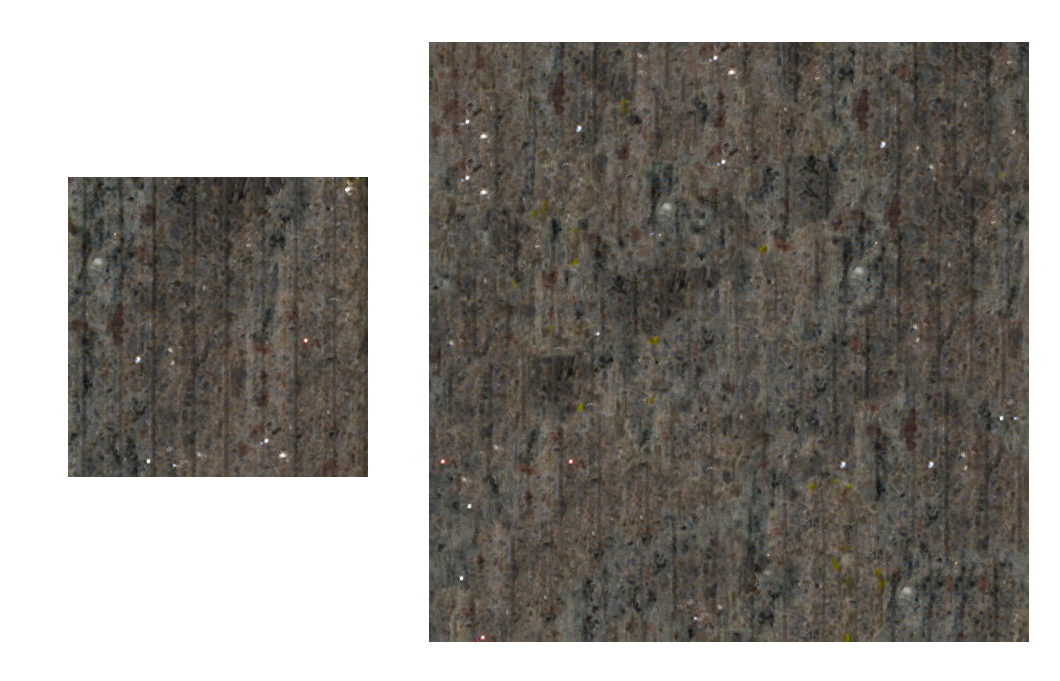
\includegraphics[width=0.75\textwidth]{figures/granite}
\end{center}
\caption{A synthesized TSV-BRDF using STAF factors as channels from initial experiments.}
\label{Fig:Granite}
\end{figure}

\section{Conclusion and Future Work}
We studied approaches addressing time-varying materials. We successfully reconstructed samples from the STAF database. We did initial experiments with the texture synthesis algorithm, see Figure~\ref{Fig:Granite}. We use the core of algorithm from the StyLit project~\cite{Fiser2016}. We plan to study issues mentioned above in detail to do TSV-BRDF synthesis in correct way. 

\bibliographystyle{plain}
\bibliography{reference}

\end{document}

